\documentclass[a4paper]{article}
\usepackage{amsmath}
\usepackage{amsthm}
\newtheorem{thm}{Theorem}
\usepackage[english]{babel}
\usepackage[utf8]{inputenc}
\usepackage{graphicx}
\usepackage[colorinlistoftodos]{todonotes}
\setlength\parindent{0pt}
\usepackage[margin=0.7in]{geometry}
\usepackage{xspace}
\usepackage[normalem]{ulem}
\usepackage{wrapfig}
\usepackage{program}


\title{Omnet Router Specification}

\newcommand{\TU}{transaction unit\xspace}
\newcommand{\vls}[1]{{\color{blue} \textbf{Vibhaa:} {#1}}}
\newcommand{\TUs}{transaction units\xspace}
\newcommand{\NewPara}[1]{\noindent{\bf #1}}

%\author{Vibhaa Sivaraman}

\date{\today}
\begin{document}
\maketitle

\section{Transaction Unit}
Each \TU is a small amount of payment that is to be sent from one end-point to another. The route for a \TU is pre-specified by the sending end-point.
Thus, each \TU contains 6 fields: amount, time sent, sender, receiver, route, priority class. A \TU should never have an amount that is larger than a pre-defined {\em{Maximum Transaction Unit}}.
The route should have the sender and the receiver as the first and last entries. For starters, we don't assume deadlines on the completion of a \TU. As and when that is added, that 
can be added as a field. \vls{Add deadlines/priority explanation}

\section{Flow of Transaction Units - Simplistic Model}
\subsection{Overview}
The high level flow per transaction unit is as follows. Let's consider a transaction arriving at router $A$ and meant to be sent out on the $A-B$ channel. When a \TU is received at 
$A$ whose next hop is $B$, we first check if there is already a queue of \TUs waiting to be sent out to $B$. If so, we add this new \TU (let's say $t$) to it. If not, we check 
if there were sufficient funds available to send out $t$. If not, we add $t$ to the queue and are done for this transaction unit. If there are funds available, 
we update the balances (decrement) on $A$'s end for the $A-B$ channel. When $B$ receives the same \TU, it increments its balance on the $A-B$ channel. Note that this naturally introduces a delay
in the balance update because of ``propagation delay'' of the \TU. If this balance increment frees up any funds for further \TUs currently queued at $B$, they should be sent out on the $B-A$ channel.

Once $B$ has completed the updates for the $A-B$ channel for the original \TU $t$, it looks at the next hop and repeats the procedure on the outgoing channel at $B$.

This is illustrated in the following flowchart.
\begin{figure}[h]
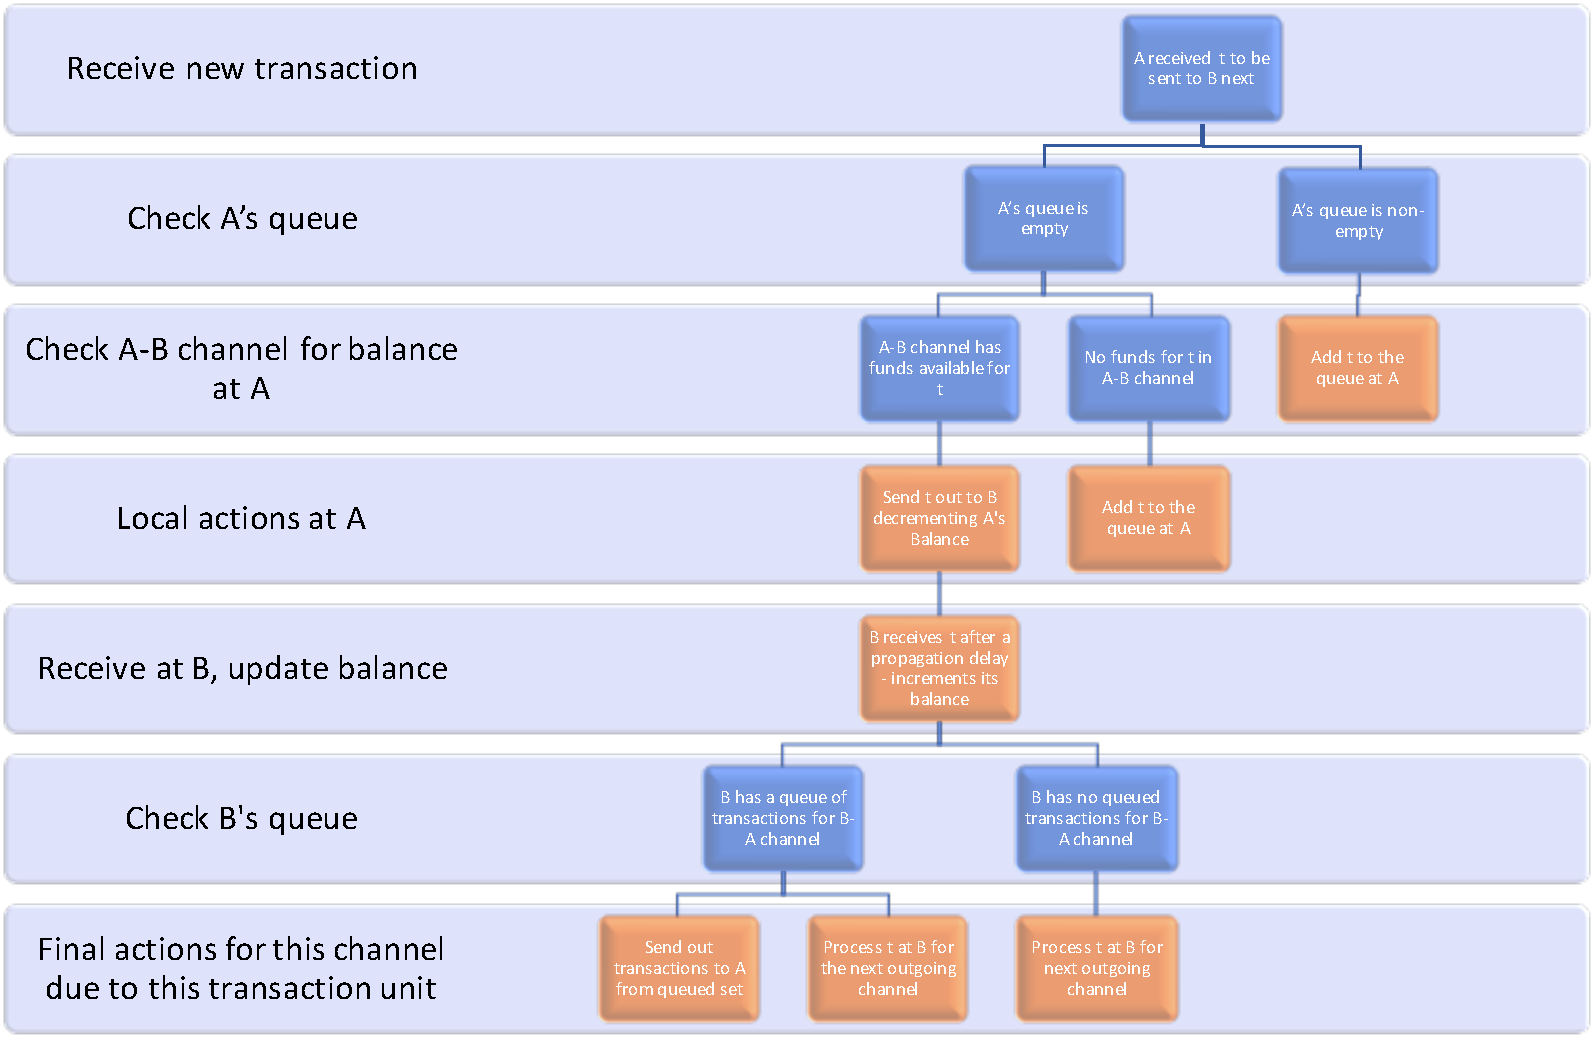
\includegraphics[width=\linewidth,height=10cm]{router_flow.pdf}
\caption{flow of transactions at a router}
\label{fig:routerflow}
\end{figure}

\subsection{Message Types}
We only have one message corresponding to a \TU.
\begin{itemize}
            \item Amount
            \item Time sent
            \item Original Sender
            \item Receiver
            \item Route
            \item Priority Class

\end{itemize}

\subsection{State Per Router}
This necessiates the following states at a router and the ability to update them
\begin{itemize}
    \item Router state (Map to identify channels): key is neighboring router id (typically public key) and value is a unique channel index or id. 
        The idea is that you would use this to identify the channel id when you have the route of a packet in terms of hops/routers it traverses. Once you have this id,
        you can use it to index into a table that contains every channel's state (described below).
    \item Per channel state:
        \begin{itemize}
            \item Balance for oneself and for the other party
            \item Queue of \TUs (in the above example, it would be a queue at A of \TUs it wanted to send to B but didn't have funds for)
      \end{itemize}
\end{itemize}


\subsection{Event Handlers for a Single Router}
This follows from the flowchart above. 
\begin{itemize}
    \item Receipt of a transaction $t$: 
        \begin{itemize}
            \item Increment balance for self by t.amount on the incoming channel and decrement other party's balance
            \item Check if any transactions were queued for the incoming channel (in the opposite direction) that can now be sent out because of the increment in balance
            \item Send as many as you can in priority order on that incoming channel
        \end{itemize}
    \item Process transaction $t$:
        \begin{itemize}
            \item Inspect next hop for $t$, map it to right outgoing channel id using the channel - channel id map per router
            \item Check if there's already transactions queued for that channel in the per channel queue
            \item If there's already queue just add $t$ to the queue for the outgoing channel
            \item If there isn't a queue, check if we have sufficient funds for $t$. If not, again, queue $t$
        \end{itemize}
    \item Send transaction $t$:
        \begin{itemize}
            \item Decrement balance for outgoing channel and increment other party's balance
            \item Send message on the outgoing channel (assume some propagation delay after which it will be received there)
        \end{itemize}
\end{itemize}








\section{Flow of HTLCs - With Receiver Acknowledgements}
\subsection{Overview}
\NewPara{Sending out HTLCs} The high level flow per HTLC is as follows. Let's consider a HTLC arriving at router $A$ and meant to be sent out on the $A-B$ channel. When a HTLC is received at 
$A$ whose next hop is $B$, we first check if there is already a queue of HTLCs waiting to be sent out to $B$. If so, we add this new HTLC (let's say $t$) to it. If not, we check 
if there were sufficient funds available to send out $t$. If not, we add $t$ to the queue and are done for this HTLC for now. If there are funds available, 
we update the balances (decrement) on $A$'s end for the $A-B$ channel. So far, this is similar to the previous simplistic model. 

However, while this means that the HTLC has been attempted on this channel and is going out from $A$ to $B$, it hasn't been cleared yet. So, we add $t$ to a set of the inflight
outgoing HTLCs which represents the set of HTLCs that have been attempted but not cleared yet. When $B$ receives the same HTLC, it adds $t$ to a set of inflight incoming HTLCs 
(that have been received but haven't been cleared yet). Note that this naturally introduces a delay in adding $t$ to the HTLCs at $B$.
This is because of ``propagation delay'' of the HTLC. During this time, the total capacity of the channel is a little less than the original capacity because only one node knows
about the HTLC $t$ (roughly similar to before). Once $B$ has completed this, it looks at the next hop and repeats the procedure on the outgoing channel at $B$. $B$ does nothing further
on the $A-B$ channel for this HTLC until an {\em{ack}} is received.

\bigskip

\NewPara{Responding to Successful Acks} Now, once the HTLC has been received at the destination node, this node will relay a successful {\em{ack}} backwards along the route of the transaction which will effectively clear 
the transactions from the ``inflight HTLC'' queues on individual routers for each channel. For instance, when $B$ receives a successful ack for some HTLC
$t$ from a neighbor node $C$, it must first remove $t$ from the set of inflight outgone HTLCs. It doesn't need to update
any balance information since the balance was already decremented. $B$ sends a balance update to $C$ to tell $C$ that it has reliably decremented the balance. ($C$ can now remove $t$ from its incoming pending HTLCs and 
increment its balance accordingly).
$B$ sends the ack to $A$ which sent the HTLC in the first place to $B$. Once it has received a balance update from $A$ for transaction $t$, $B$ clears $t$ from
the set of inflight incoming HTLCs and increments its view of the $A-B$ balance accordingly.

\bigskip

\NewPara{Failure Acks} (Can wait on this) Now, once a given node has decided to fail an HTLC, it can relay a failure {\em{ack}} backwards along the route of the transaction which will effectively clear 
the transactions from the ``inflight HTLC'' queues on individual routers for each channel all the way up. For instance, when $B$ receives a failure ack for some HTLC
$t$ from a neighbor node $C$, it must first remove $t$ from the set of inflight outgone HTLCs. It also needs to update its balance information since the balance was already decremented. 
$B$ sends the ack to $A$ which sent the HTLC in the first place to $B$. $B$ also clears $t$ from
the set of inflight incoming HTLCs since it can't complete.


This is illustrated in the following flowchart.
\begin{figure}[h]
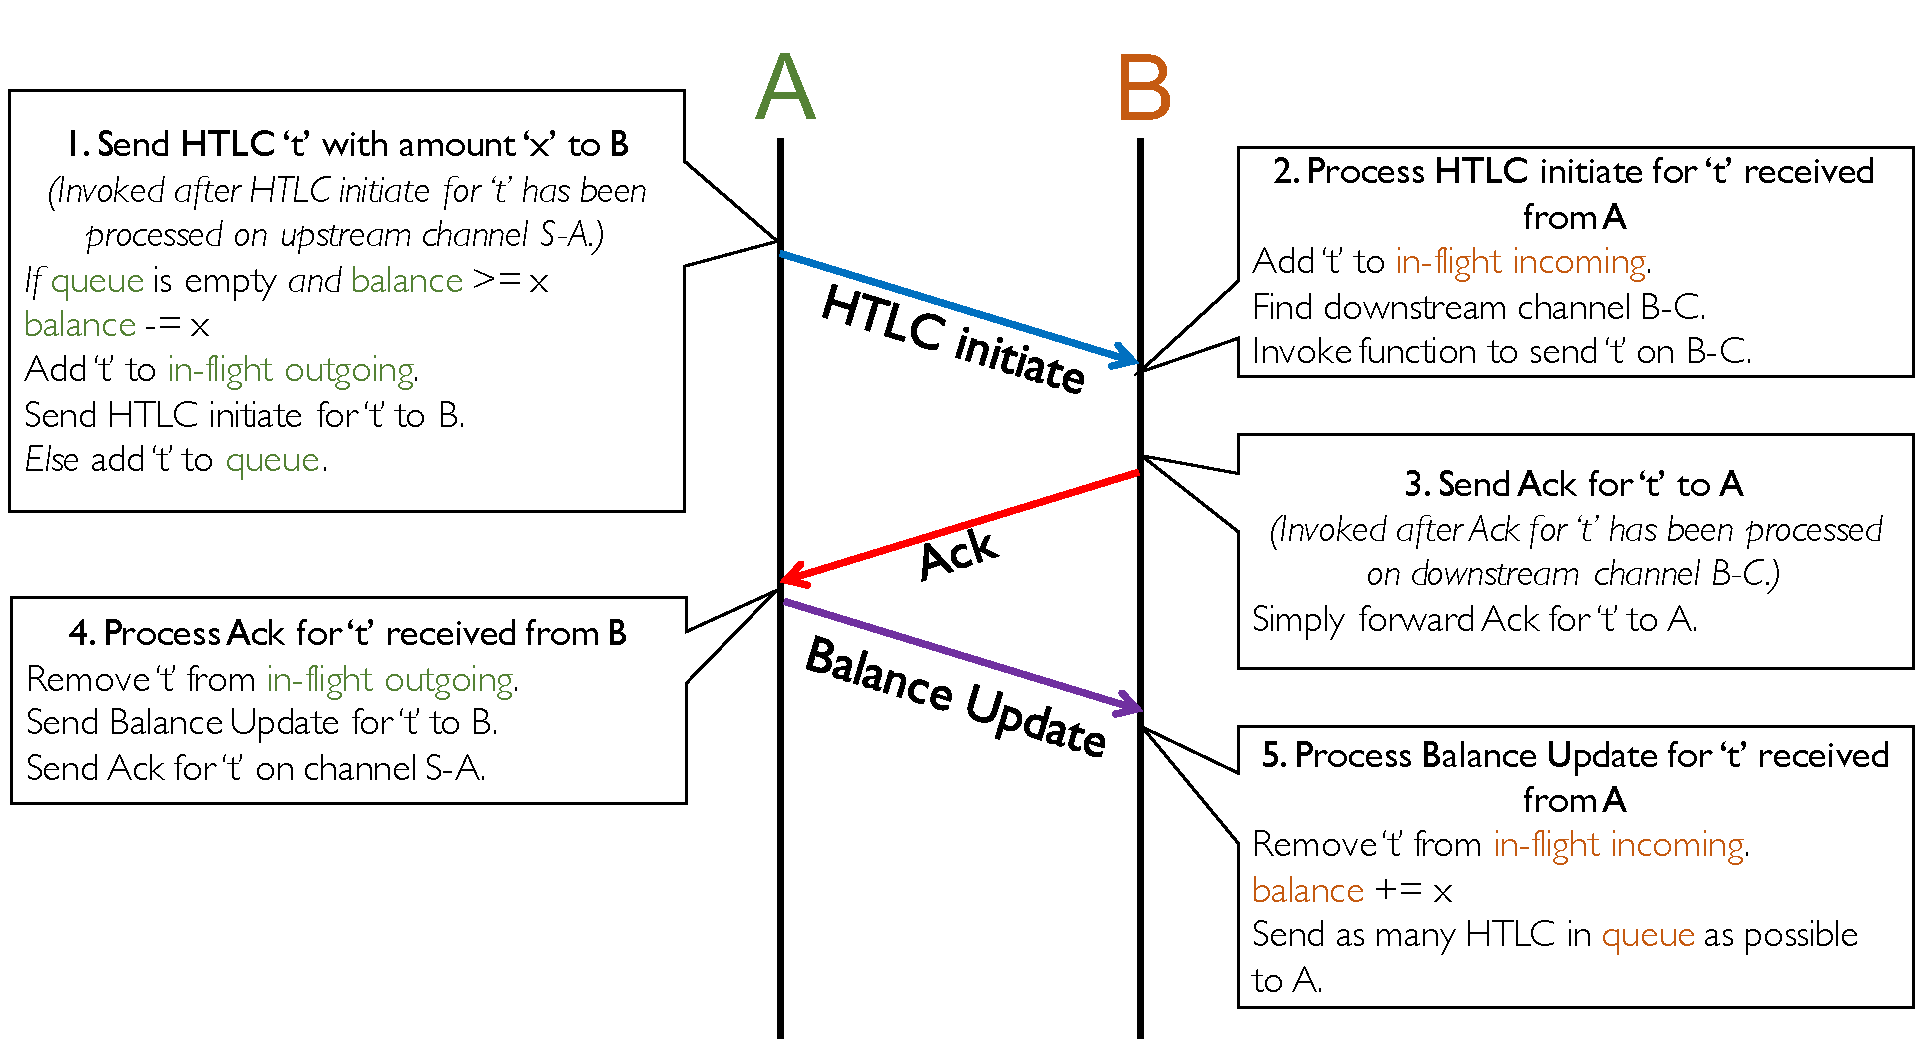
\includegraphics[width=\linewidth,height=10cm]{htlcAckFlow.pdf}
\caption{flow for a given HTLC $t$ at a given channel}
\label{fig:htlcflow}
\end{figure}


\subsection{Message Types}
\begin{itemize}
    \item HTLC Initiate: This is similar to the current transaction message
        \begin{itemize}
            \item Amount
            \item Time sent
            \item Original Sender
            \item Receiver
            \item Route
            \item Priority Class
            \item Transaction id (needed for removing it from the set of inflight transactions)
        \end{itemize}

    \item HTLC Ack
        \begin{itemize}
            \item Transaction id for which the Ack is received
            \item Route for the ack (reverse of the path the transaction was sent on
            \item Status (Success or Failure) - just in case we want to simulate failures and propagate them upwards
            \item Secret - Dummy field for now (might never change)
        \end{itemize}

    \item Balance Update
        \begin{itemize}
            \item Transaction id that is being completed (Assuming that the inflight transaction set at each node has the amount already, this is all we really need to update the balances correctly)
            \item Local Balance (The one who is sending the message)
            \item Other Party's balance (the one the message is sent to)
        \end{itemize}
\end{itemize}

\subsection{State Per Router}
This necessiates the following states at a router and the ability to update them
\begin{itemize}
    \item Router state (Map to identify channels): key is neighboring router id (typically public key) and value is a unique channel index or id. 
        The idea is that you would use this to identify the channel id when you have the route of a packet in terms of hops/routers it traverses. Once you have this id,
        you can use it to index into a table that contains every channel's state (described below).
    \item Per channel state:
        \begin{itemize}
            \item Balance for oneself \sout{and for the other party}
            \item Total Channel Capacity
            \item Queue of \TUs (in the above example, it would be a queue at A of \TUs it wanted to send to B but didn't have funds for)
            \item Inflight transactions that were sent out on this channel - hashmap with transaction ids as keys and amount as value
            \item Inflight transactions that came into this channel - hashmap with transaction ids as keys and amount as value
        \end{itemize}
\end{itemize}

\subsection{Event Handlers for a single Router}
This follows from the flowchart above. 
\begin{itemize}
    \item Receipt of an incoming incomplete HTLC $t$ from upstream router: 
        \begin{itemize}
            \item Add $t$ and the amount to incoming inflight transaction set
             \item Process HTLC $t$:
                \begin{itemize}
                    \item Inspect next hop for $t$, map it to right outgoing channel id using the channel - channel id map per router
                    \item Check if there's already transactions queued for that channel in the per channel queue
                    \item If there's already queue just add $t$ to the queue for the outgoing channel
                    \item If there isn't a queue, check if we have sufficient funds for $t$. If not, again, queue $t$
                \end{itemize}
            \item Send HTLC $t$ to downstream router:
                \begin{itemize}
                    \item Decrement balance for outgoing channel \sout{don't yet increment other party's balance}
                    \item Add $t$ and the amount to outgoing inflight transaction set
                    \item Send ``HTLC Initiate'' message on the outgoing channel (assume some propagation delay after which it will be received there)
                \end{itemize}
        \end{itemize}
    \item Receive HTLC $t$'s ack from downstream router:
        \begin{itemize}
            \item Successful ack:
                \begin{itemize}
                    \item Remove $t$ from outgoing inflight transaction set on (me - downstream) router channel
                    \item Send ``balance update'' message to the downstream router with your own balance decremented and the other router's incremented
                    \item \sout{Increment your local view of the other party's balance}
                    \item Send ``HTLC ack'' to upstream router
                \end{itemize}
            \item Failure Ack:
                \begin{itemize}
                    \item Remove $t$ from outgoing inflight transaction set and (only) increment my side of the balance
                    \item Send ``Failure HTLC ack'' to upstream router
                    \item Remove $t$ from incoming inflight transaction set for the corresponding channel it came in on
                \end{itemize}

        \end{itemize}
    \item Receipt of balance update
        \begin{itemize}
            \item Increment my side of the balance by the corresponding amount \sout{and decrement other party's}.
            \item Check if any transactions were queued for the incoming channel (in the opposite direction) that can now be sent out because of the increment in balance
            \item Send as many as you can in priority order on that incoming channel

        \end{itemize}
\end{itemize}

\section{Waterfilling Algorithm}
\subsection{Heuristic Idea}
The essence of the waterfilling algorithm is to maintain balance across a fixed set of paths by always trying to send on the path(s) with maximum bottleneck balance
in the direction that you want to send. The bottleneck balance is defined as the minimum balance amongst the edges or payment channels on the path from the source
to the destination. For instance, if you have the following payment channel network (Fig.~\ref{fig:sample_graph}), the bottleneck balances on $P_1$, $P_2$, $P_3$ and $P_4$ between $s$ and $t$
are 20, 15, 10 and 5.

\begin{wrapfigure}[14]{L}{0.3\textwidth}
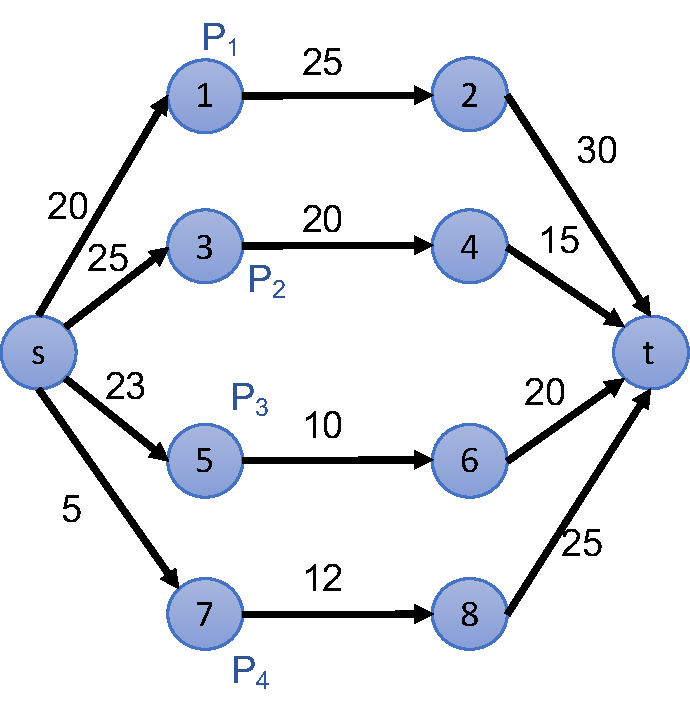
\includegraphics[height=4.5cm]{sample_graph.pdf}
\caption{Numbers on edges denote the balance in that direction on the payment channel}
\label{fig:sample_graph}
\end{wrapfigure}

If one had to send a payment of $18$ units, the first $5$ would be sent on $P_1$, the next $10$ would be sent equally on $P_1$ and $P_2$ (with $5$ on each) and the
last $3$ would be sent one each on paths $P_1$, $P_2$ and $P_3$. If the payment isn't fully completed in this process, any remaining amount is queued at the sender
until the deadline on the sender for the payment expires.

\subsection{Simulation Overview}
Inferring the bottleneck balances is not a trivial task since nodes don't have a global view of every other node/payment channel balance. Thus, this algorithm
breaks down into two phases: querying for channel balances and processing of the probes to compute the waterfilling splits. These two phases will run at slightly different time scales. The querying/probing will happen on every RTT; we send out a probe immediately after receiving the response from the previous one. 
We start these probes the only once we receive a payment that is to be sent out to that recipient and stop once there is no more demand/transaction to be sent
to avoid unnecessary probing overhead. The computation of the splits happens as necessary when the next \TU to send arrives or a current set of splits complete/fail.

\subsection{Message Types}
\begin{itemize}
    \item Query Channel Balance
        \begin{itemize}
            \item Sender
            \item Receiver
            \item Path 
            \item Is this probe on the reverse path and coming back?
            \item Current Hop Number (starts at 0 when the sender creates this message)
            \item Empty Map of node to channel balance on the outgoing channel from that node along the path
        \end{itemize}


    \item Modification to HTLC Initiate/ACK/Balance update:
        \begin{itemize}
            \item Additional sequence number to identify what chunk of the original transaction this is
        \end{itemize}

\end{itemize}

\subsection{Processing Channel Balance Query at every node}
\begin{itemize}
    \item The sender is reponsible for creating this probe message for every path that it wants to probe and initialize the fields including the empty map

    \item Every intermediate node on the forward path (check by checking is the flag for reverse path is set to {\em{false}}) 
        is responsible for (a) ensuring that it is on the path (at index denoted by hop number), (b) finding
        the balance on the (me - nextHop) channel and adding it to the map and (c) forwarding the probe to the next hop. 
    \item When the probe is received at the receiver, it changes the direction of the probe by changing the path field to the reverse of the original. 
        The hop number needs to be reset to $0$ and the reverse path flag to {\em{true}}.

    \item Every intermediate node (along the path) on the reverse direction merely forwards the probe and doesn't need to do anything else. An added check is to
        verify that the current node is on the path (at the index denoted by hop number) and then forward it to the next hop (denoted by the item at the next index
        on the path)
\end{itemize}

\subsection{New State}
\begin{itemize}
    \item State Per Sender
        \begin{itemize}
            \item Per destination state (updated/initialized when a probe is received)
                \begin{itemize}
                    \item Destination
                    \item Set of paths (let's start with $2$ shortest edge disjoint paths)
                    \item Bottleneck balance on each of those paths
                \end{itemize}
            \item Set of pending transactions (some of these might have been partially completed relative to the initial amount they started with) along with the last sequence
                number that was used for each of them. This must be updated every time a new transaction is split or an old one is coalesced due to a failure.
        \end{itemize}
    
    \item State Per Receiver
        \begin{itemize}
            \item Transaction Id of transactions received
            \item Set of sequence numbers for the given transaction id that have been already received/acked successfully.
        \end{itemize}

\end{itemize}

\subsection{Event Handlers for a Sender}
\begin{itemize}
    \item Receipt of completed probe
        \begin{itemize}
            \item Update the information in the per-destination table with the latest bottleneck balance for that path
            \item Involves computing the minimum across all the balances on that path
        \end{itemize}

    \item New Transaction To Send
        \begin{itemize}

            \item If this is a brand new transaction (Sequence number - $0$), first send out a probe and wait for the response.
            \item Look up the corresponding set of paths for that destination and the associated bottleneck balances. 
            \item Compute the splits for that transaction according to the balances on each of those paths. This means, send as much as you can on the path with highest bottleneck balance 
                until its balance falls to the second highest one. Then send equal amounts on the two highest bottleneck balance paths until their balances fall to the third and so on. 
		
		\begin{program}
                \mbox{Computes output path\_list which consists of tuples (path, amount on path)}
		\BEGIN \\ %
                  |path_list| := \emptyset
                  ~\\
		  \FOR i:=1 \TO k \DO
		     B_i := |compute_bottleneck_bal|(P_i)\\ PQ := PQ \cup (P_i, B_i); %
		\rcomment{Insert balances into some heap PQ}
		\END \\
                ~\\

                \DO \IF |size|(PQ) > 0 \AND |txn_amt| > 0	    
		  |highest_bal| := |PQ.poll()| % 
		  \rcomment{Let the path with this highest balance be $p_{max}$}\\
		  |second_highest_bal| := |PQ.peek()|\\
		  |diff_to_send| := |highest_bal| - |second_highest_bal|\\% 
                  |amt_to_send| := min(|txn_amt|/(|size|(|path_list|) + 1), |diff_to_send|)
		 
                  ~\\
                  \FOR p \  |in| \ |path_list| \DO
		    |amt|_p := |amt|_p + |amt_to_send|
		    |txn_amt| := |txn_amt| - |amt_to_send|
		  \END
                  ~\\

		  |path_list| := |path_list| \cup (p_{max}, |amt_to_send|)
		\END
            \END

		\end{program}

            \item Create separate transactions with those splits that are then sent on each of the paths. Give each of them a unique sequence number incrementing from the last one used or starting
                from 1.

            \item If the payment is not completed in the process, queue the remaining at the sender for trying later into the set or queue that is tracking pending payments.
        \end{itemize}

    \item Received feedback from a payment that was attempted
        \begin{itemize}
            \item Successful Ack: Do nothing. When splitting the payment, we already assumed it would go through and only queued up the remaining amount.
            \item Failure Ack: Add the failed amount to the pending transaction set. If there was already something associated with this transaction, coalesce the two by just adding the failed amount to it.
            \item Treat any remaining part of the parent transaction that this Ack was a part of as a new transaction and follow the above procedure.

        \end{itemize}
\end{itemize}
\section{Time Outs with no Splitting of Transactions}
\subsection{Overview}
The purpose of handling timeouts is a way for the sender to cancel a previously sent transactions at time $t$ and be guaranteed that the transaction has been successfully canceled or receive a successful ack by time $t+delta$. A new message type $timeOutMsg$ is introduced that is generated at initialization by the sender of the transaction and is sent out at the $timeSent + timeOutLimit$  for each transaction. A message type $clearStateMsg$ is introduced at every router node that periodically implements the effects of the $timeOutMsg$.

\subsection{New Message Types}
\begin{itemize}
    \item timeOutMsg
    \begin{itemize}
        \item Amount
        \item Transaction Id
    \end{itemize}
    \item clearStateMsg
    \begin{itemize}
        \item (possibly $delta$, else no fields)
    \end{itemize}
\end{itemize}
\subsection{New State per Node}
\begin{itemize}
    \item set of tuples containing transaction id for time out messages and time stamp for when time out message was received at the router node as well as the previous and next nodes if applicable 
\begin{itemize}
    \item \begin{verbatim} set<canceledTrans> canceledTransactions \end{verbatim}
    \item \begin{verbatim} canceledTrans \end{verbatim}
    \begin{itemize}
        \item \begin{verbatim}transactionId \end{verbatim}
        \item  \begin{verbatim}simTime_t\end{verbatim} of time we received timeOutMsg 
        \item \begin{verbatim}prevNode  \end{verbatim} (if not sender)
        \item \begin{verbatim}nextNode \end{verbatim} (if not destination)
    \end{itemize}
\end{itemize} 
\item (Host only)  set of transaction ids for transactions that we have received acks for and also have a time out limit (so we already generated a timeOutMsg and scheduled it for that transaction)
\begin{itemize}
    \item \begin{verbatim} set<int> successfulDoNotSendTimeOut; \end{verbatim}
\end{itemize}


\end{itemize}
\subsection{Implementation}
\subsubsection{ Changes to initialization}
    \begin{itemize}
        \item Calculate the longest path between two nodes in the graph, store as a global constant $delta$
    \end{itemize}

\subsubsection{ Handling the timeOutMsg}
    \begin{itemize}
        \item (Generation) a timeOutMsg is generated at initialization by the sender of the transaction and is scheduled to arrive at the same sender node at time $timeSent + timeOutLimit$  for each transaction
        \item if the timeOutMsg is at hop count 0 or the sender (first time we are seeing it), check if the transaction Id is in the set of successful transactions (successfulDoNotSendTimeOut), if so, then delete the timeOutMsg, and the transactionId from the set of successful transactions
        \item If not, when processing the timeout message at other routers, 
        \begin{itemize}
            \item add the transaction id and current time to the set of canceled transactions (canceledTransactions)
            \item if the time out message is at the destination node, delete it
        \end{itemize}
    \end{itemize}
\subsubsection{ Changes to Handling Ack Message}
    \begin{itemize}
        \item check if the transaction id in the ack message is in the set of canceled transactions. If so, delete it from the set of canceled transactions.
        \item (Host) if the ack message is back at the original sender of the transaction, add the transaction to the set of successful transaction ids (successfulDoNotSendTimeOut)

    \end{itemize}
\subsubsection{ Changes to Handling Transaction Messages}
    \begin{itemize}
        \item when receiving a transaction message, check to see if the transaction Id is in the set of canceled transactions, if so, delete the transaction message.
        \item \sout{ when processing transactions (these include transactions in the queue, sending the transactionMsg out and decrementing the balance), check if the transaction we are trying to send out is in the set of canceled transactions, if so, delete it and don’t change any balances}

    \end{itemize}
\subsubsection{ Handling clearStateMsg}
    \begin{itemize}
        \item (Generation) a message is generated at initialization for every node (router/sender) scheduled to arrive at time  currentTime+clearRate
        \item For all transactions in the set canceled transactions whose cancellation time  was more than $delta$ time ago, remove the transaction from the incoming and outgoing maps. If removed from outgoing map, increment my end of the balance on the payment channel to the next node. If removed from the incoming queue, we do $not$ need to decrement the balance to the previous node. Search for the transaction in the queue of transactions waiting to be sent to the next node, and delete it if found.
        \item Delete the transaction mentioned from the set of canceled transactions. 
    \end{itemize}

\section{Handling Time Outs with split transaction (Waterfilling)}
\subsection{Overview}
We add the "acked amount" to the ack messages and keep track of the total amount sent on each path, and total amount acked on each path, for every transaction. A transaction is successful only if total amount acked (across all paths) is same as transation amount. Otherwise, we send a timeout message on paths where the difference between total amount sent and total amount acked is non-zero.

\subsection{Additional data structures}
\begin{itemize}
    \item maintain a map with the key as transaction id and index of one of k paths and the value as a two numbers, the total amount sent down that path, and the total amount we have received acknowledgements for from that path
    \begin{itemize}
        \item \begin{verbatim}map<tuple<int, int>, AmtState> transPathToAmtState \end{verbatim}
        \item struct AmtState
            \begin{itemize}
                \item double amtSent
                \item double amtReceived
            \end{itemize}
    \end{itemize}
\end{itemize}
\subsection{Changes to handling timeOutMessages}
\begin{itemize}
    \item Generate a timeOutMsg for each of the k paths. When the timeOutMsg arrives at time timeSent + timeOutLimit, check if the map value corresponding the transaction id and path index has the same value for amount sent and amount acknowledged. If not, forward the timeOutMsg.
\end{itemize}
\subsection{Changes to handling acks}
\begin{itemize}
    \item When an ack is received at the sender, get the transaction id and path index from the ack, and update the map transPathToAmtState
\end{itemize}


\end{document}



